%%% PgDay 2011
%%%
%%% PostgreSQL 9.1 features extensibility to the next level. While this
%%% often is a concern for C-developers among us, this talk will detail why
%%% extensions are a first-class facility for anyone doing Stored
%%% Procedures, whatever their implementation language.
%%%
%%% If you ever did type CREATE OR REPLACE FUNCTION, be it in LANGUAGE SQL,
%%% then you're in!

\documentclass[english]{beamer}
\usepackage[utf8,latin9]{inputenc}
%%\usepackage[latin9]{inputenc}
\usepackage[T1]{fontenc}
\usepackage{babel}

\usepackage{beamerthemesplit}
\usetheme{Amsterdam}
\beamertemplatetransparentcovered

\title{Extensions are good for business logic}
\subtitle{Beamer Theme: Amsterdam}
\author{Dimitri Fontaine}
\date{Oct 20, 2011}

\begin{document}

\frame{\titlepage}

\frame{
  \frametitle{Extensions?  Logic?  Fuzzy Business?  Say what?}
  \tableofcontents[pausesections]
}

\section{Extensions and Business Logic}

\subsection{What's an Extension?}

\frame{
  \frametitle{Extensions}

  \begin{description}
  \item<1->[Extensions] PostgreSQL is very extensible, and with \alert{full
    support} now. Almost all about SQL solving is possible to implement as
    an extension.

  \item<2->[Full Support] Wait, I wish you were here
    \begin{itemize}
    \item Stuttgart, December 2010, PgDay
    \item Brussels, February 2011, FOSDEM
    \item Ottawa, May 2011, PgCon
    \end{itemize}

  \item<3->[Featuring] dump \& restore, versioning, upgrades, dependencies
  \end{description}
}

\begin{frame}[fragile]
  \frametitle{Some extensions example}

  \begin{center}
    46 Contribs, Community extensions, Private ones...
  \end{center}

\begin{columns}[c]

\column{.18\textwidth}
  \begin{itemize}
   \item cube
   \item ltree
   \item citext
   \item \alert{hstore}
   \item intagg
  \end{itemize}

\column{.25\textwidth}
  \begin{itemize}
   \item adminpack
   \item \alert{pgq}
   \item pg\_trgm
   \item wildspeed
   \item \alert{dblink}
  \end{itemize}

\column{.22\textwidth} 
  \begin{itemize}
   \item \alert{PostGIS}
   \item ip4r
   \item temporal
   \item prefix
   \item pgfincore
  \end{itemize}

\column{.41\textwidth}
  \begin{itemize}
   \item pgcrypto
   \item pg\_stattuple
   \item pg\_freespacemap
   \item pg\_stat\_statements
   \item \alert{pg\_standby}
  \end{itemize}

\end{columns}
\end{frame}

\begin{frame}[fragile]
  \frametitle{Some extensions are simpler than that}

  For the sake of this talk, if you have some \textit{business logic
    functions} in your database, you have an extension. Even \texttt{VIEW}
  qualifies.

\begin{example}[Very simple extension]
\begin{verbatim}
  CREATE OR REPLACE FUNCTION accounting.vat(numeric)
   RETURNS numeric
   LANGUAGE SQL
  AS $$
    RETURN $1 * 0.196;
  $$;
\end{verbatim}
\end{example}
\end{frame}

\subsection{MVC: Where's the Model}

\frame{
  \begin{center} 
    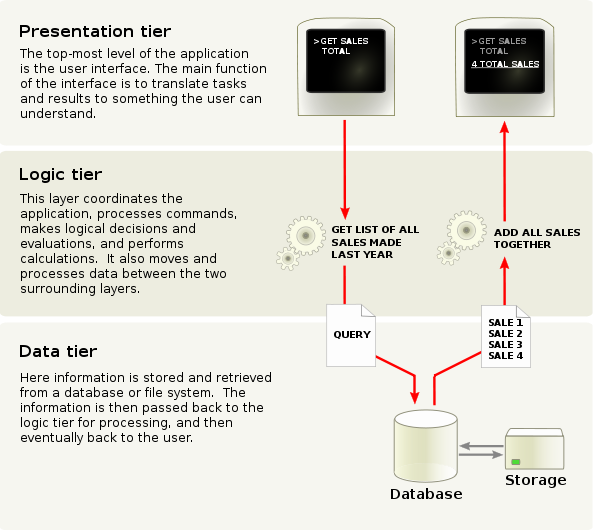
\includegraphics[height=2.8in]{tiers.png}
  \end{center}   
}

\frame{
  \frametitle{Put the logic into the database layer}

  \begin{center} 
    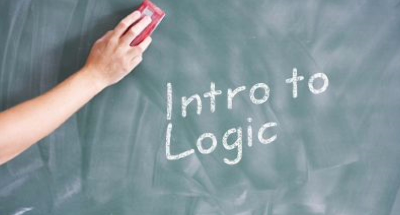
\includegraphics[height=2.2in]{logic.png}
  \end{center}   
}

\subsection{Packaging your in database Model}

\begin{frame}[fragile]
  \frametitle{35.15. Packaging Related Objects into an Extension 1/6}

\begin{example}[pair--1.0.sql]
\begin{verbatim}
CREATE TYPE pair AS ( k text, v text );

CREATE OR REPLACE FUNCTION pair(anyelement, text)
RETURNS pair LANGUAGE SQL AS 'SELECT ROW($1, $2)::pair';

CREATE OR REPLACE FUNCTION pair(text, anyelement)
RETURNS pair LANGUAGE SQL AS 'SELECT ROW($1, $2)::pair';

CREATE OR REPLACE FUNCTION pair(anyelement, anyelement)
RETURNS pair LANGUAGE SQL AS 'SELECT ROW($1, $2)::pair';

CREATE OR REPLACE FUNCTION pair(text, text)
RETURNS pair LANGUAGE SQL AS 'SELECT ROW($1, $2)::pair;';  
\end{verbatim}
\end{example}
\end{frame}

\begin{frame}[fragile]
  \frametitle{35.15. Packaging Related Objects into an Extension 2/6}

\begin{example}[pair--1.0.sql]
\begin{verbatim}
CREATE OPERATOR ~> (LEFTARG = text, RIGHTARG = anyelement,
                    PROCEDURE = pair);
CREATE OPERATOR ~> (LEFTARG = anyelement, RIGHTARG = text,
                    PROCEDURE = pair);
CREATE OPERATOR ~> (LEFTARG = anyelement, RIGHTARG = anyelement,
                    PROCEDURE = pair);
CREATE OPERATOR ~> (LEFTARG = text, RIGHTARG = text,
                    PROCEDURE = pair);
\end{verbatim}
\end{example}
\end{frame}

\begin{frame}[fragile]
  \frametitle{35.15. Packaging Related Objects into an Extension 3/6}

  PostgreSQL needs some \textit{metadata} about your extension, fill in the
  \texttt{control} file.

\begin{example}[pair.control]
\begin{verbatim}
# pair extension
comment = 'A key/value pair data type'
default_version = '1.0'
relocatable = true
\end{verbatim}
\end{example}
\end{frame}

\begin{frame}[fragile]
  \frametitle{35.15. Packaging Related Objects into an Extension 4/6}

  To easy the package installation process, you need a scary
  \texttt{Makefile}. Beware of \texttt{VPATH}, he's your friend, but he's
  very picky about it.

\begin{example}[Makefile]
\begin{verbatim}
EXTENSION = pair
DATA = pair--1.0.sql # avoid $(wildcard sql/*--*.sql)

PG_CONFIG = pg_config
PGXS := $(shell $(PG_CONFIG) --pgxs)
include $(PGXS)
\end{verbatim}
\end{example}
\end{frame}

\begin{frame}[fragile]
  \frametitle{35.15. Packaging Related Objects into an Extension 5/6}

  Now, relax and profit.

\begin{example}[psql]
\begin{verbatim}
CREATE EXTENSION pair SCHEMA utils;
\end{verbatim}
\end{example}
\end{frame}

\begin{frame}[fragile]
  \frametitle{35.15. Packaging Related Objects into an Extension 6/6}

  Oh, and maybe you wanted to use the extension, too.

\begin{example}[psql]
\begin{verbatim}
CREATE TABLE foo(kv pair);
INSERT INTO foo(kv)
     SELECT 'x' ~> 'y';
\end{verbatim}
\end{example}
\end{frame}

\section{Managing upgrades}

\subsection{Extension upgrades}

\begin{frame}[fragile]
  \frametitle{Upgrading an extension}

  That used to be a ``guru'' only operation...

\begin{example}[extension update]
\begin{verbatim}
ALTER EXTENSION pair UPDATE;
ALTER EXTENSION pair UPDATE TO '1.1';

SELECT * FROM pg_available_extensions();
SELECT * FROM pg_available_extension_versions();
\end{verbatim}
\end{example}
\end{frame}

\subsection{From development to production}

\begin{frame}[fragile]
  \frametitle{Packaging upgrades in development}

\begin{example}[update to 1.4]
\begin{verbatim}
  ALTER EXTENSION pair UPDATE TO '1.1';
  ...
  ALTER EXTENSION pair UPDATE TO '1.4';
\end{verbatim}
\end{example}

  \begin{itemize}
   \item<1-> \texttt{pair---1.0.sql}
   \item<2-> \texttt{pair---1.0---1.1.sql}
   \item<3-> \texttt{pair---1.1---1.2.sql}
   \item<3-> \texttt{pair---1.2---1.3.sql}
   \item<3-> \texttt{pair---1.3---1.4.sql}
  \end{itemize}
\end{frame}

\begin{frame}[fragile]
  \frametitle{Packaging upgrades for production rollouts}

\begin{example}[update to 1.4]
\begin{verbatim}
  ALTER EXTENSION pair UPDATE TO '1.4';
\end{verbatim}
\end{example}

  \begin{itemize}
   \item<1-> \texttt{\char`\\dx} shows we're at version \texttt{1.0}
   \item<1-> PostgreSQL will happily apply those files:
   \item<2-> \texttt{pair---1.0---1.1.sql}, \texttt{pair---1.1---1.2.sql},
   \item<2-> \texttt{pair---1.2---1.3.sql}, \texttt{pair---1.3---1.4.sql}
   \item<3-> \alert{Check} with \texttt{pg\_available\_extension\_versions()}!
  \end{itemize}
\end{frame}

\subsection{Managing Rollouts}

\frame{
  \frametitle{Packaging upgrades for production rollouts}

  Sometimes playing each step one after the other is not what you want.

  \begin{itemize}
   \item<1-> Prepare \texttt{pair---1.0---1.4.sql}
   \item<2-> PostgreSQL will happily prefer this file
   \item<3-> Check with \texttt{pg\_available\_extension\_versions()}
  \end{itemize}
}

\section{Conclusion}

\subsection{Any question?}

\begin{frame}[fragile]
  \frametitle{Any question?}

  \begin{center}
    Now is a pretty good time to ask!
  \end{center}

  \linebreak
  \begin{center}
    If you want to leave feedback, consider visiting
    \url{http://2011.pgconf.eu/feedback}
  \end{center}
\end{frame}

\end{document}
